
\section{Integration of a new device}\label{app:new_device}

Both Vire  and MOS systems are  designed to be expandable  in terms of
device integration.  This section  decribes the  integration of  a new
device in the \emph{Control and Monitoring System}.

\subsection{Integration of a new device in the MOS environment}

Any new device is described through  a dedicated XML model file.  This
XML  file  is  created  from  a  template  file  elaborated  from  the
\emph{interface control document} (ICD) and associated to the model of
the  device. The  format  of the  XML  file is  described  in the  MOS
(Multipurpose OPCUA Server) User Guide. % ref

Typically, a device is embedded in a OPCUA server and implemented as a
OPCUA  \emph{simple  device}.   The  OPCUA server  itself  is  located
through an unique dedicated IP address and port.

The simple device  instance, hosted in the OPCUA  server, may contains
other sub-devices and/or \emph{datapoints}.   It is thus considered as
the root  of a hierarchy  of daughter  objects at deeper  levels.  The
daughter objects (devices or datapoints) are named relatively to their
top level  parent device. Figure  \ref{fig:an:mos_dev_1} shows an
example of a device embedded in a MOS server.

\begin{figure}[h]
\begin{center}
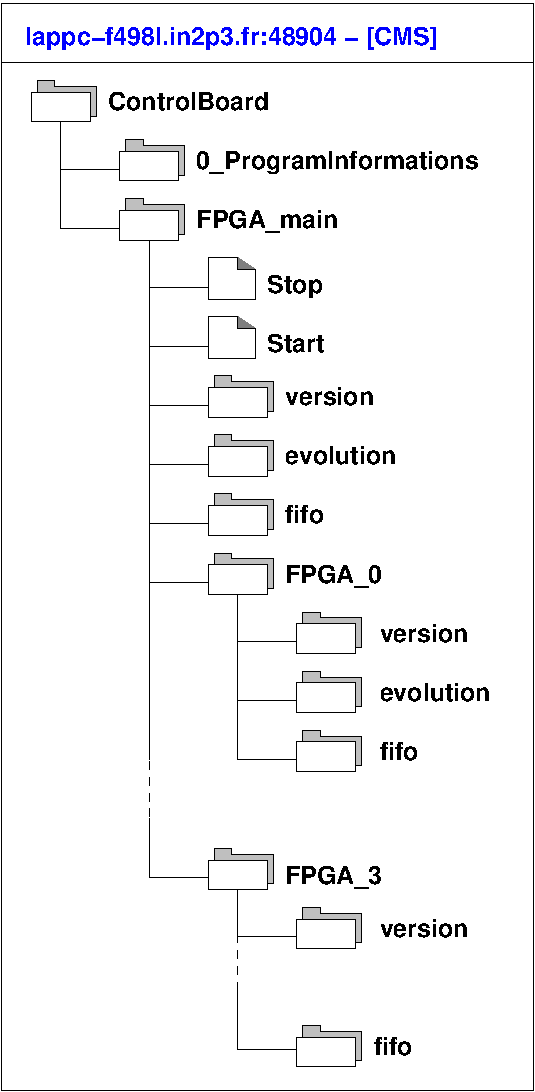
\includegraphics[width=5cm]{appendix/images/MOS_device_example_1.pdf}
\end{center}
\caption{Example of a  device managed through a MOS  server.  The root
  device is named \texttt{ControlBoard}.  First level daughter devices
  are  \texttt{0\_ProgramInformations} and  \texttt{FPGA\_main}.  Here
  the          MOS/OPCUA          server          is          labelled
  \texttt{CMS}.}\label{fig:an:mos_dev_1}
\end{figure}

% TODO


\subsection{Integration of a new device in the Vire environment}

The Vire  API also implements a  mechanism to describe a  hierarchy of
devices.  This  mechanism is independant  of the  one used in  the MOS
system but can  be easily made compatible with it.   This means that a
MOS  hierarchy  of devices  can  be  represented  in Vire.   The  Vire
hierarchy of  devices can  be considered as  some kind  of filesystem,
each device  being a folder with  its unique path, as  shown on figure
\ref{fig:an:mos_dev_2}.   The \emph{methods}  associated to  a devices
(or a datapoint) can be considered as plain executable files stored in
the  device's folder  : they  constitute the  set of  \emph{resources}
associated to the device.


\begin{figure}[h]
\begin{center}
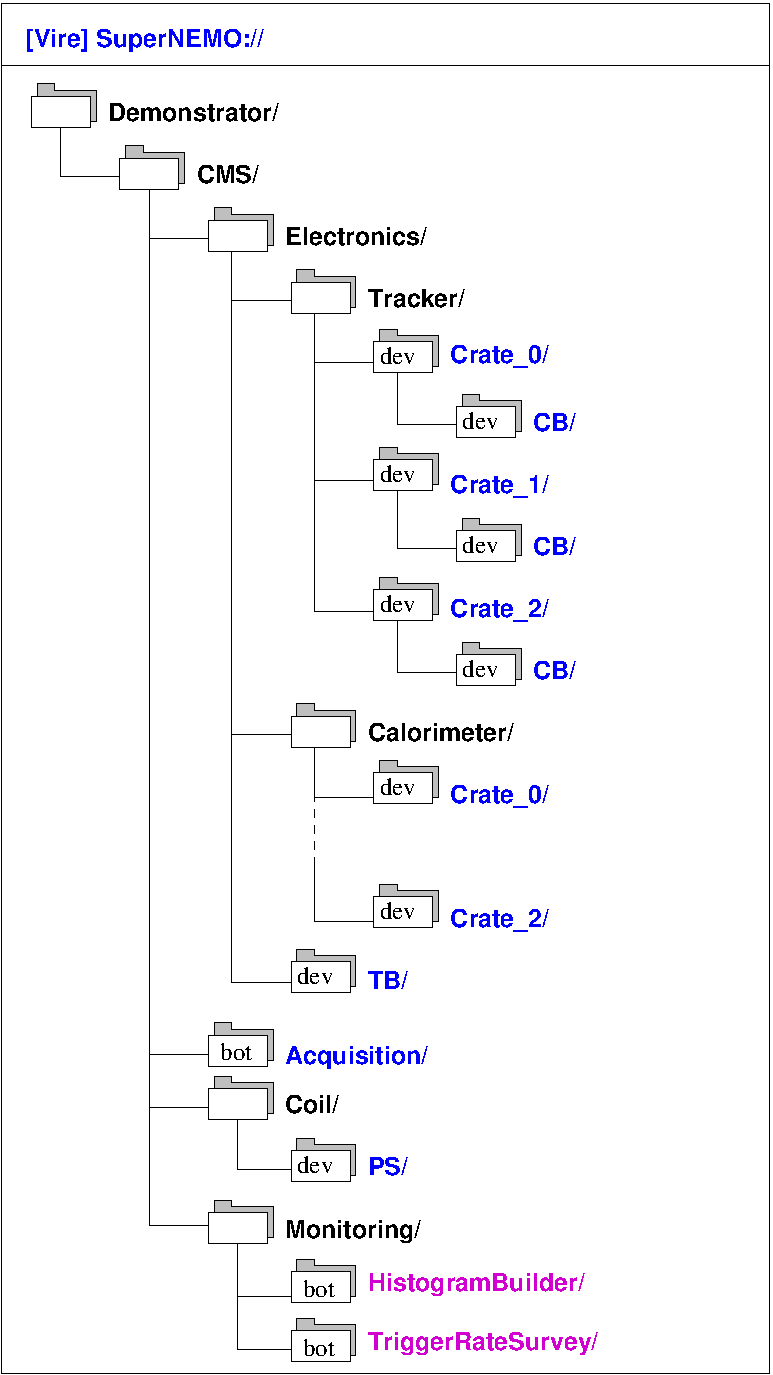
\includegraphics[width=5cm]{appendix/images/MOS_device_example_2.pdf}
\end{center}
\caption{Example of a hierarchy of  devices described by the Vire API.
  The root device is named  \texttt{SuperNEMO:}.  The top level (root)
  device  is  named  \texttt{Demonstrator}.  The  devices  colored  in
  \textcolor{blue}{blue}  are managed  through MOS/OPCUA.  The devices
  colored in \textcolor{magenta}{magenta} are directly embedded in the
  Vire server.  Devices with the \texttt{dev} tag are typical hardware
  device.  Devices  with the  \texttt{bot}  tag  are typical  software
  devices.   The  devices  colored in  \textbf{black}  are  structural
  pseudo-devices used to organize and  present a comprehensive view of
  the hierarchy. }\label{fig:an:mos_dev_2}
\end{figure}

The organisation of this hierarchy of devices is arbitrary and defined
by the designer of the  \emph{Control and Monitoring System}.  What is
important  to  understand  is  that  some  of  these  devices  can  be
associated  to  \emph{hardware  devices}  (a  power  supply  crate,  a
temperature probe\dots) and others  can be \emph{pseudo-devices}, i.e.
pure   software  object   (a   monitoring  robot,   a  file   transfer
daemon\dots).

In the context of the coupling of  the Vire server and the CMS server,
we are  in the event that  some devices are managed  by some MOS/OPCUA
servers and others are managed  in the Vire server itself.  Typically,
\emph{hardware devices}  are systematically managed through  the OPCUA
technology.  Vire has a mechanism to integrate such devices in its own
hierarchy.  This mechanism can  be considered like the \emph{mounting}
of   a   remote   filesystem   from  a   local   filesystem.    Figure
\ref{fig:an:mos_dev_0} illustrates  the case of many  hardware devices
-- managed by MOS -- that are integrated in the Vire system.  From the
Vire point of  view, the user does not see  the implementation details
for such  devices. He  does not  know the identity  of the  MOS server
hosting the device. He does not even know if the device is hosted by a
MOS server.  Devices are simply visible through the standard hierarchy
published by Vire with its  own device naming scheme, regardless their
true location.



\begin{figure}[h]
\begin{center}
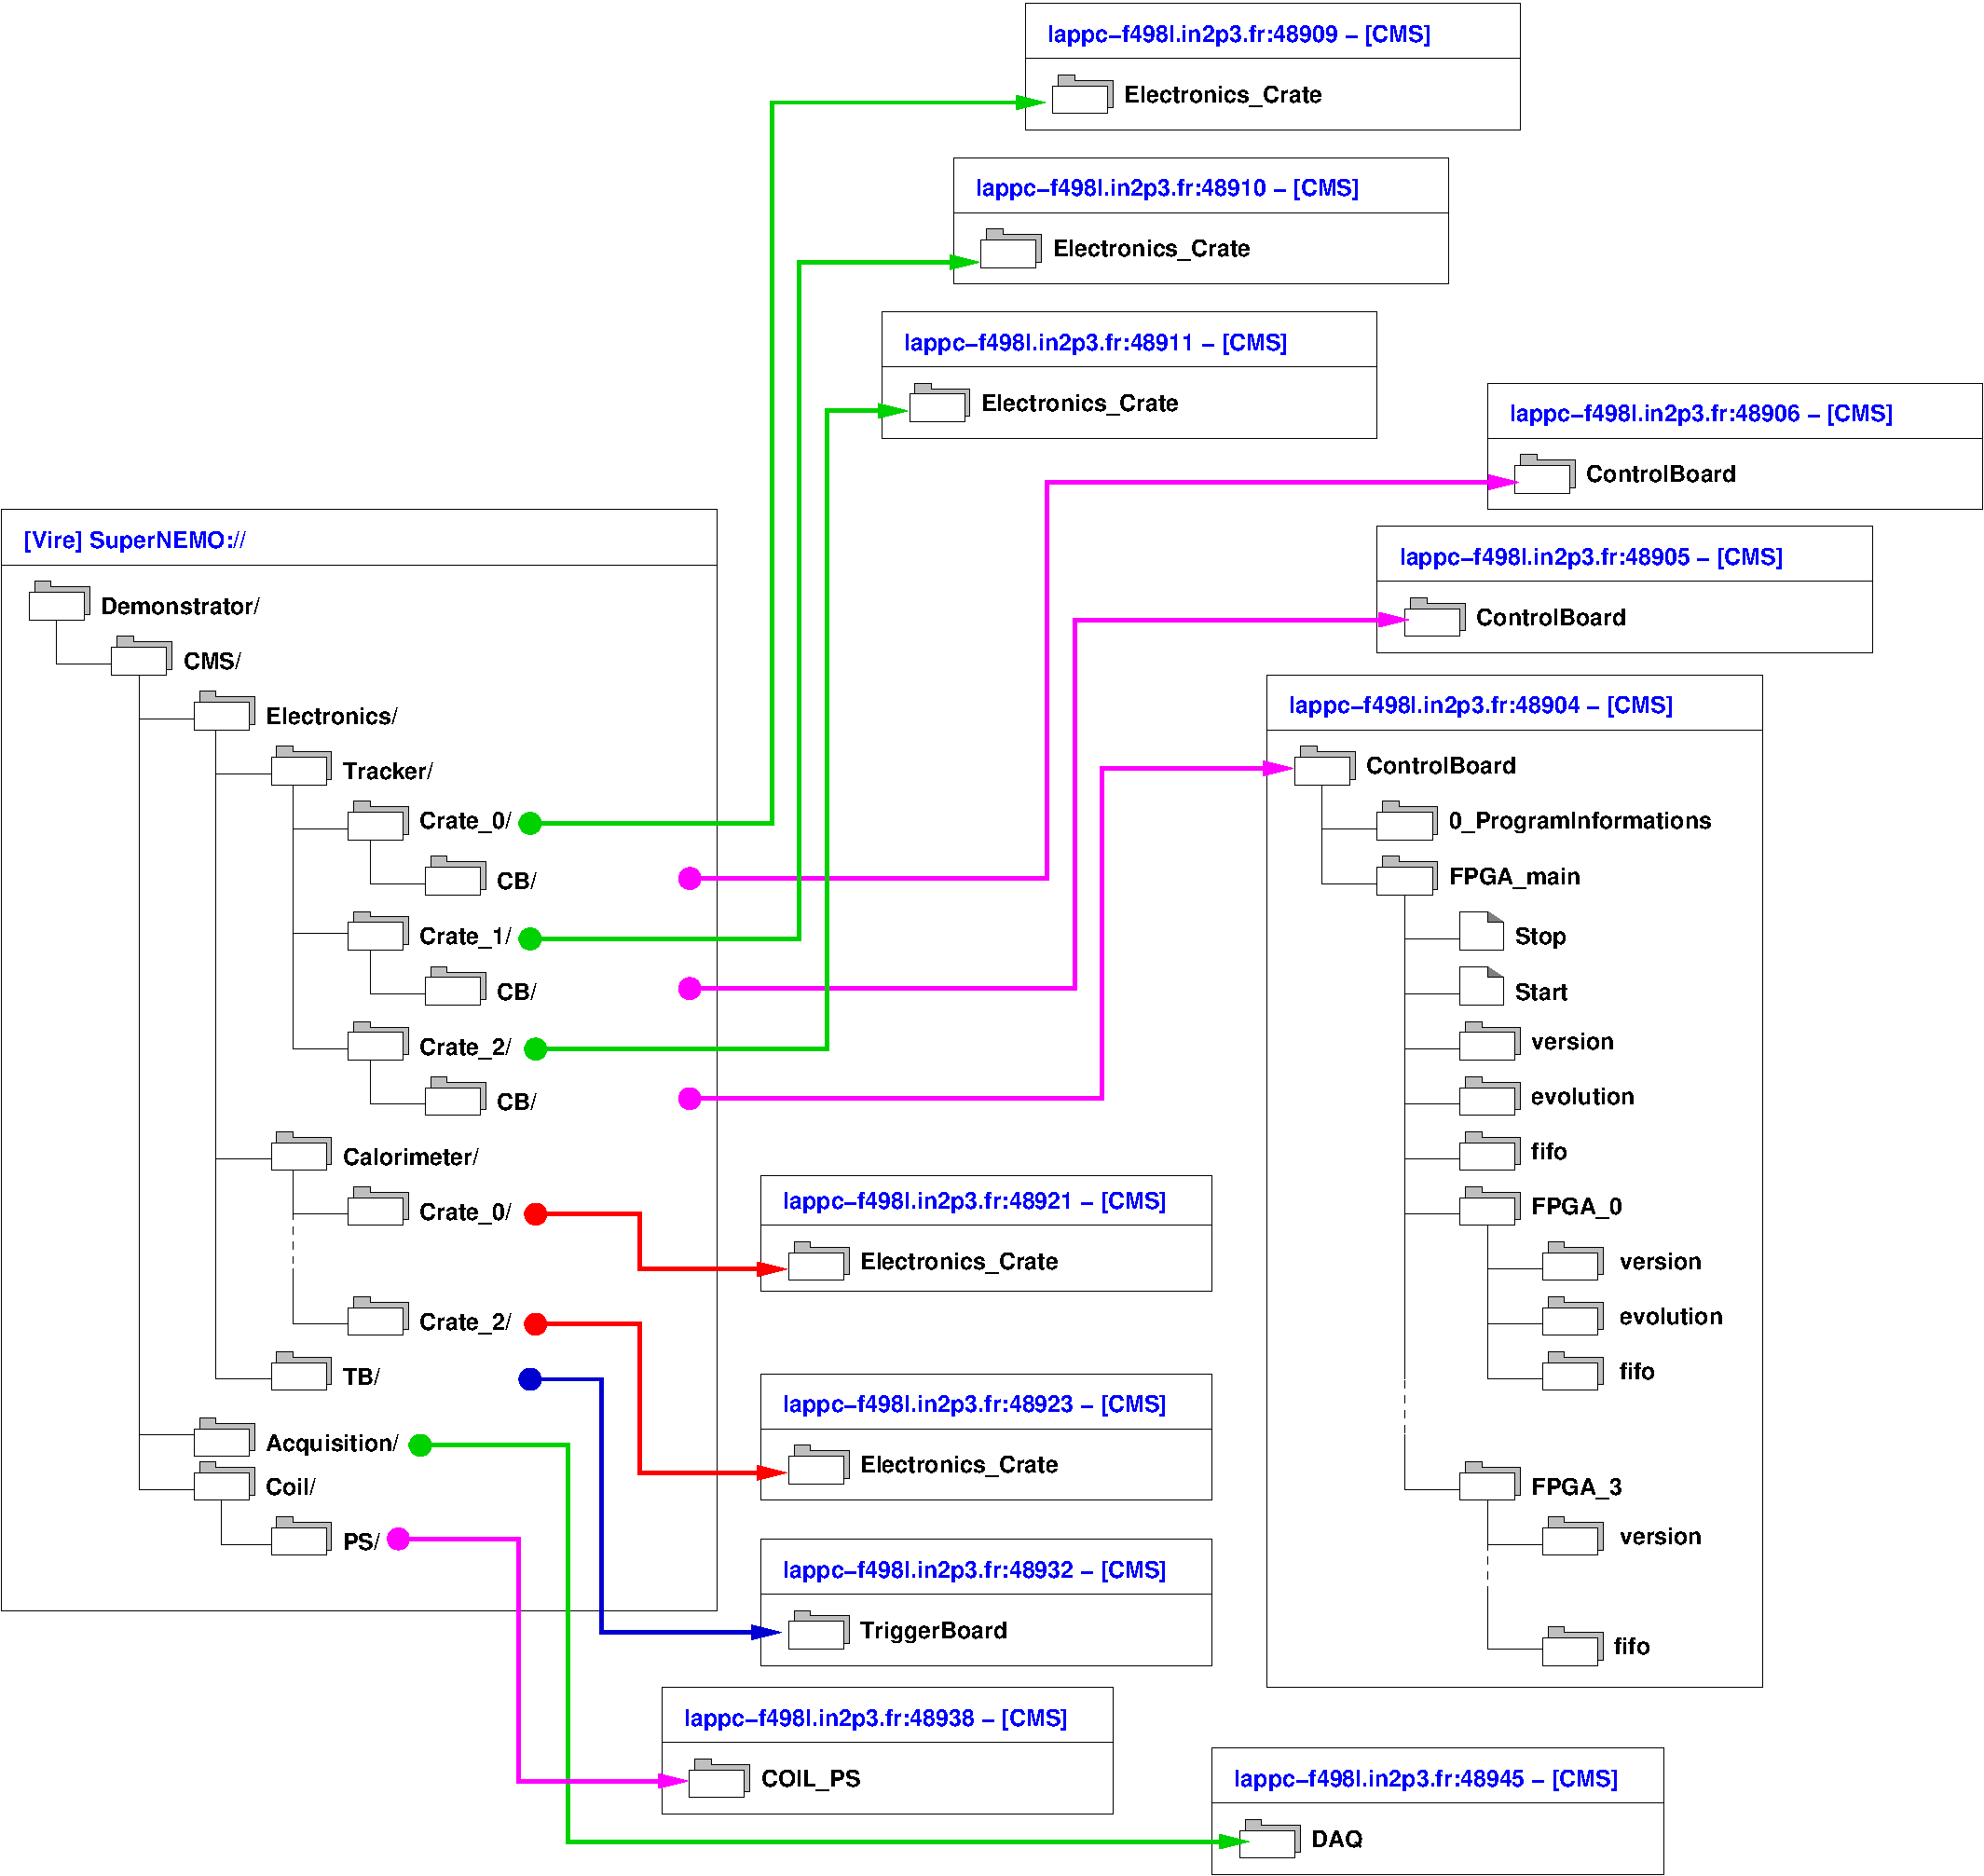
\includegraphics[width=\linewidth]{appendix/images/MOS_device_example_0.pdf}
\end{center}
\caption{The  mounting of  many  MOS device  hierarchies  in the  Vire
  device hierarchy.  Each OPCUA server  runs a simple  hardware device
  that is \emph{mounted} from a specific node with its own path.
%% of  devices described by the Vire API.
%%   The root device is named  \texttt{SuperNEMO:}.  The top level (root)
%%   device is  named \texttt{Demonstrator}. The devices  colored in blue
%%   are managed  through MOS/OPCUA. The  devices colored in  magenta are
%%   directly embedded in the Vire server.  Devices with the \texttt{dev}
%%   tag are typical  hardware device. Devices with  the \texttt{bot} tag
%%   are typical software devices.
}\label{fig:an:mos_dev_0}
\end{figure}




\subsection{Example}

Using  the examples  displayed  in  figure \ref{fig:an:mos_dev_0},  we
consider  in detail  the way  one specific  device managed  by MOS  is
mounted   in  the   Vire   hierarchy.  Figure   \ref{fig:an:mos_dev_3}
illustrates the mounting of a MOS device in Vire.

Here the Vire  server publishes the path of a  device representing the
control board  of the third  electronic crate  for the tracker  of the
SuperNEMO demonstrator module.  The full Vire path of this device is:

\textcolor{blue}{\texttt{SuperNEMO://Demonstrator/CMS/Electronics/Tracker/Crate\_2/CB}}

This is  the only Vire identifier  recognized by user to  address this
device.

On    the   figure,    one    can   see    that    the   MOS    server
\texttt{lappc−f498l.in2p3.fr} (port 48904) hosts a simple device which
is locally named \texttt{ControlBoard}.

When  mounting   this  device  in   the  Vire  hierarchy,   the  local
\texttt{[CMS]}  namespace and  \texttt{ControlBoard} device  names are
hidden and replaced by the Vire device path.  All daughter devices and
datapoints of  the \texttt{CMS/ControlBoard} device are  integrated as
daughters        of        the         Vire        device        named\\
\texttt{SuperNEMO://Demonstrator/CMS/Electronics/Tracker/Crate\_2/CB}.


For example, the \texttt{FPGA\_main} daughter device is now associated
to the following Vire path:

\textcolor{blue}{\texttt{SuperNEMO://Demonstrator/CMS/Electronics/Tracker/Crate\_2/CB/FPGA\_main/}}

and  its  \texttt{Stop} method  is  automatically  addressed with  the
following \emph{leaf} path:

\textcolor{blue}{\texttt{SuperNEMO://Demonstrator/CMS/Electronics/Tracker/Crate\_2/CB/FPGA\_main/Stop}}


\begin{figure}[h]
\begin{center}
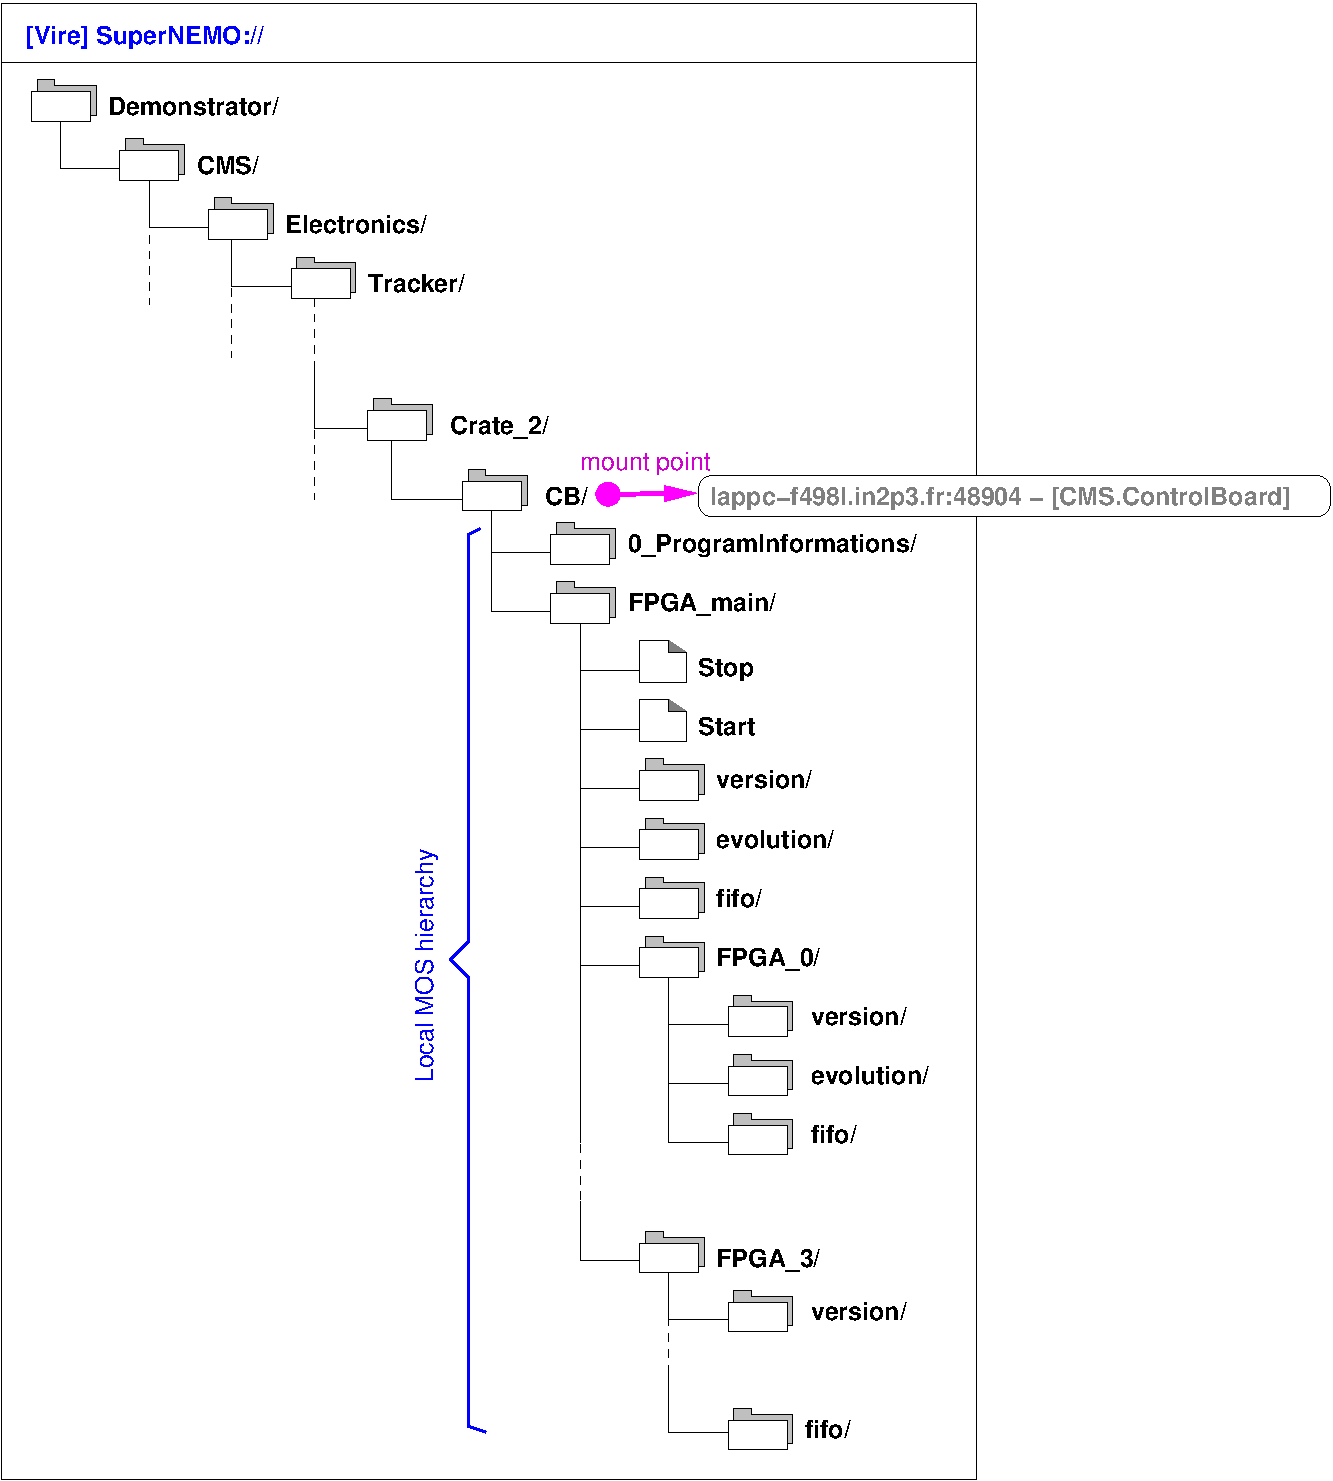
\includegraphics[width=0.8\linewidth]{appendix/images/MOS_device_example_3.pdf}
\end{center}
\caption{The  mounting of  one  MOS device and its local hierarchy  in the  Vire
  device hierarchy.}\label{fig:an:mos_dev_3}
\end{figure}



\subsection{Vire/MOS mapping}

As it can be  seen in the above example, the integration  of a new MOS
device in the Vire system is  achieved through soem kind of filesystem
mounting operation.   Particularly, it is  shown that the MOS  name of
the   mounted  root   device  is   replaced  by   an  arbitrary   Vire
path. However, all daughter  nodes (devices, datapoints) attached from
this root  node have their  relative MOS  names preserved in  the Vire
naming scheme.

Any  resource  (method)  associated  to any  of  such  daughter  nodes
inherits this relative naming scheme.

As Vire applications  describe resources through their  Vire paths, it
is thus needed to build an explicit map that associates resource paths
to MOS address  and name. The CMS  server will be able  to resolve the
MOS server/port and  embedded device associated to  the resource path.

The goal of the \texttt{devices\_launch.conf} file is not only to tell
the CMS server what MOS server should  be loaded and ran at start, but
also  to describe  the  \emph{mounting point/names}  used  by Vire  to
access the resources associated to MOS devices.  From the informations
stored in the  file, an explicit associative array must  be built when
the Vire server connect to the CMS server.  It will play the role of a
resource path resolver  when requests about resources will  be sent by
Vire applications.  This associative array  must be locked  during the
Vire/CMS connection.



%\subsubsection{Preparation of XML device models}

%% \noindent\underline{Pre-condition:}
%% The device is working and validated through the MOS/OPCUA server

%% \begin{enumerate}

%% \item Produce XML décrivant le modèle du device enrichi
%%   des metadata
%% Rédaction du fichier XML décrivant le modèle du device

%% \item Génération des fichiers model du type de device pour Vire

%% \item Génération des fichiers instances resolv.conf

%% \end{enumerate}


\vfill
\pagebreak
\clearpage

% end
